\documentclass{article}
\usepackage{tikz}
\usepackage{amsmath}
\usepackage[paperwidth=18cm,paperheight=18cm,margin=0.5cm]{geometry}
\pagestyle{empty}
\begin{document}
\centering
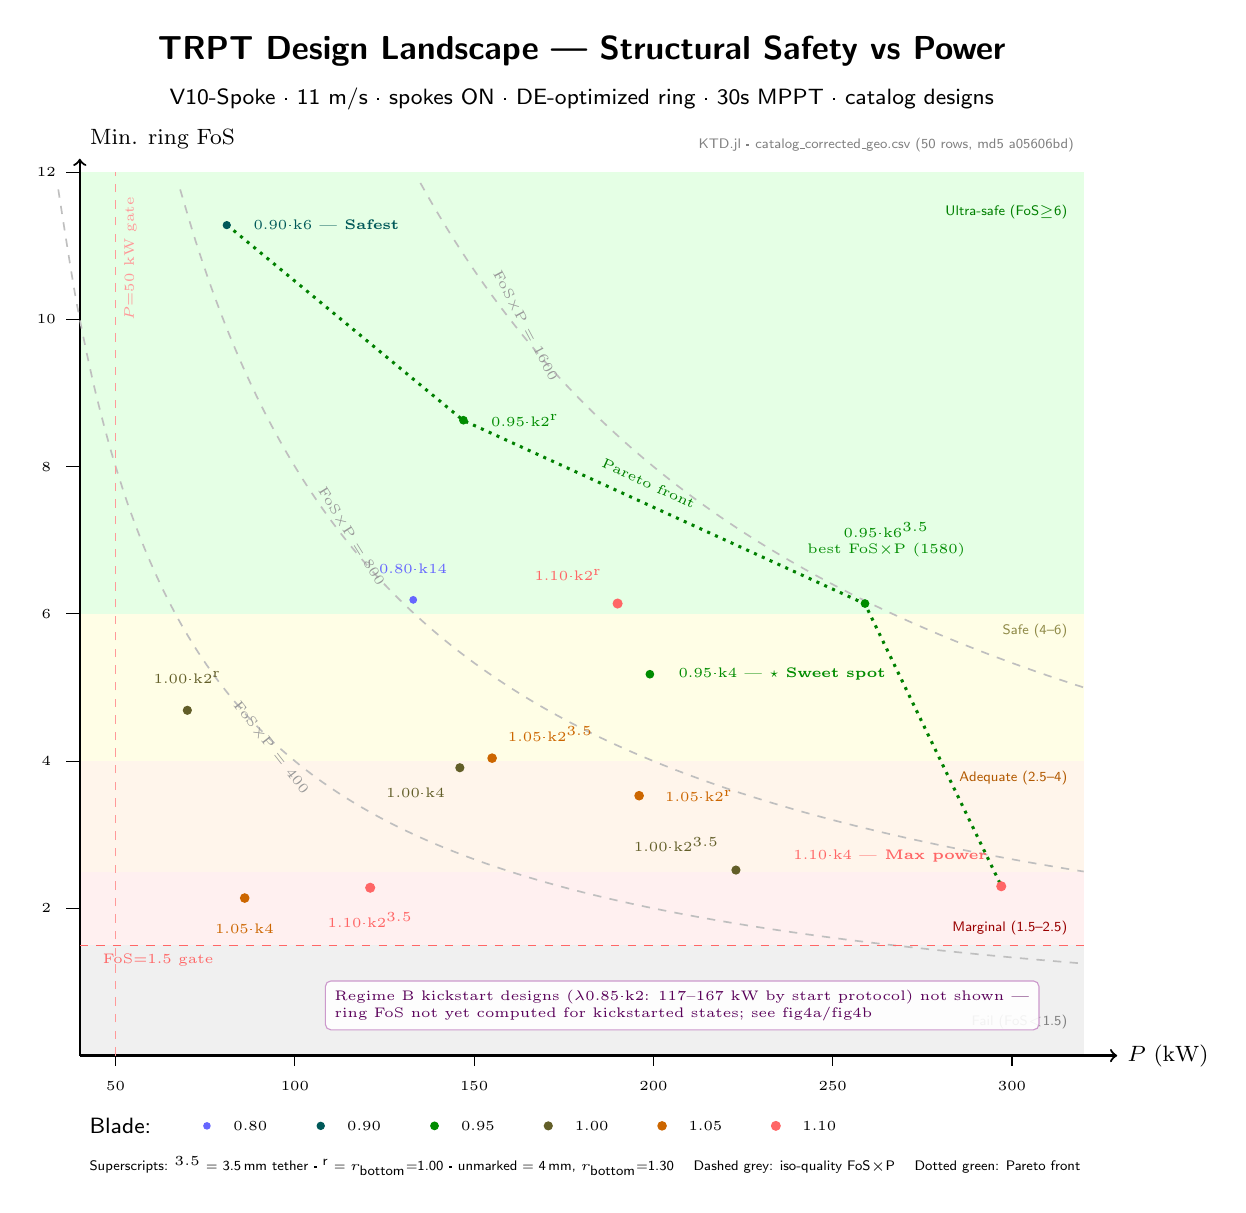
\begin{tikzpicture}[scale=0.85]

% Merged chart (2026-07-16): replaces both the old fig2 and chart-structural-efficiency.
% Adds iso-quality (FoS x P) curves + Pareto front from the latter; keeps band shading
% from the former. All 14 catalog-viable points labelled. Kickstart regime noted.

% ── Title ──
\node[font=\large\sffamily\bfseries] at (10.0, 17.0) {TRPT Design Landscape — Structural Safety vs Power};
\node[font=\footnotesize\sffamily] at (10.0, 16.3) {V10-Spoke · 11 m/s · spokes ON · DE-optimized ring · 30s MPPT · catalog designs};

% ── Coordinate maps: x = 2.5 + (P-40)/280*15,  y = 2.0 + FoS*1.1 ──

% ── FoS bands (behind everything) ──
\fill[green!10]  (2.5, 8.6)  rectangle (17.5, 15.2);   % FoS>=6 ultra-safe
\fill[yellow!10] (2.5, 6.4)  rectangle (17.5, 8.6);    % 4-6 safe
\fill[orange!8]  (2.5, 4.75) rectangle (17.5, 6.4);    % 2.5-4 adequate
\fill[red!6]     (2.5, 3.65) rectangle (17.5, 4.75);   % 1.5-2.5 marginal
\fill[black!6]   (2.5, 2.0)  rectangle (17.5, 3.65);   % <1.5 fail

% ── Axes ──
\draw[->, thick] (2.5, 2.0) -- (18.0, 2.0) node[right, font=\footnotesize] {$P$ (kW)};
\draw[->, thick] (2.5, 2.0) -- (2.5, 15.4) node[above right, font=\footnotesize] {Min. ring FoS};

% X ticks: x = 2.5 + (P-40)/280*15
\foreach \p in {50, 100, 150, 200, 250, 300} {
  \pgfmathsetmacro{\x}{2.5 + (\p-40)/280*15}
  \draw (\x, 1.85) -- (\x, 2.0);
  \node[font=\tiny] at (\x, 1.55) {\p};
}

% Y ticks
\foreach \f in {2, 4, 6, 8, 10, 12} {
  \pgfmathsetmacro{\y}{2.0 + \f*1.1}
  \draw (2.3, \y) -- (2.5, \y);
  \node[font=\tiny] at (2.0, \y) {\f};
}

% ── Iso-quality curves: FoS × P = C (structural quality) ──
\foreach \C/\pmin in {400/34, 800/68, 1600/135} {
  \draw[black!25, dashed, line width=0.6pt, domain=\pmin:320, samples=60, smooth]
    plot ({2.5 + (\x-40)/280*15}, {2.0 + min(\C/\x, 12.0)*1.1});
}
\node[font=\tiny, black!40, rotate=-52] at (5.35, 6.6)  {FoS$\times$P = 400};
\node[font=\tiny, black!40, rotate=-58] at (6.55, 9.75) {FoS$\times$P = 800};
\node[font=\tiny, black!40, rotate=-62] at (9.15, 12.9) {FoS$\times$P = 1600};

% ── Gate lines ──
\draw[dashed, red!60] (2.5, 3.65) -- (17.5, 3.65);   % FoS=1.5 gate
\pgfmathsetmacro{\gx}{2.5 + (50-40)/280*15}
\draw[dashed, red!40] (\gx, 2.0) -- (\gx, 15.2);     % P=50 gate
\node[font=\tiny, red!60, anchor=west] at (2.7, 3.42) {FoS=1.5 gate};
\node[font=\tiny, red!40, rotate=90] at ({\gx+0.22}, 13.9) {$P{=}50$ kW gate};

% ── Band labels (right edge, kept clear of points and iso-curves) ──
\node[font=\tiny\sffamily, anchor=east] at (17.4, 14.6) {\textcolor{green!50!black}{Ultra-safe (FoS$\ge$6)}};
\node[font=\tiny\sffamily, anchor=east] at (17.4, 8.35) {\textcolor{yellow!50!black}{Safe (4--6)}};
\node[font=\tiny\sffamily, anchor=east] at (17.4, 6.15) {\textcolor{orange!70!black}{Adequate (2.5--4)}};
\node[font=\tiny\sffamily, anchor=east] at (17.4, 3.9)  {\textcolor{red!60!black}{Marginal (1.5--2.5)}};
\node[font=\tiny\sffamily, anchor=east] at (17.4, 2.5)  {\textcolor{black!50}{Fail (FoS$<$1.5)}};

% ── Pareto front (non-dominated: 0.90k6 → 0.95k2r → 0.95k6-3.5 → 1.10k4) ──
\draw[green!50!black, dotted, line width=1.1pt]
  (4.70, 14.41) -- (8.23, 11.49) -- (14.23, 8.75) -- (16.27, 4.53);
\node[font=\tiny, green!50!black, rotate=-25] at (11.0, 10.55) {Pareto front};

% ── Data points: \pt{P}{FoS}{radius pt}{colour} ──
\def\pt#1#2#3#4{
  \pgfmathsetmacro{\x}{2.5 + (#1-40)/280*15}
  \pgfmathsetmacro{\y}{2.0 + #2*1.1}
  \draw[#4, fill=#4] (\x, \y) circle (#3 pt);
}

% Ultra-safe
\pt{81}{11.28}{1.5}{teal!70!black}
\node[font=\tiny, teal!70!black, anchor=west] at (4.95, 14.41) {0.90·k6 — \textbf{Safest}};
\pt{147}{8.63}{1.6}{green!55!black}
\node[font=\tiny, green!55!black, anchor=west] at (8.5, 11.49) {0.95·k2$^{\text{r}}$};
\pt{133}{6.19}{1.4}{blue!60}
\node[font=\tiny, blue!60, above] at (7.48, 9.05) {0.80·k14};
\pt{190}{6.14}{1.9}{red!60}
\node[font=\tiny, red!60, above left] at (10.45, 8.95) {1.10·k2$^{\text{r}}$};
\pt{259}{6.14}{1.6}{green!55!black}
\node[font=\tiny, green!55!black, above, align=center] at (14.55, 9.3) {0.95·k6$^{3.5}$\\best FoS$\times$P (1580)};

% Safe
\pt{199}{5.18}{1.6}{green!55!black}
\node[font=\tiny, green!55!black, anchor=west] at (11.3, 7.70) {0.95·k4 — $\star$ \textbf{Sweet spot}};
\pt{70}{4.69}{1.7}{olive!60!black}
\node[font=\tiny, olive!60!black, above] at (4.11, 7.42) {1.00·k2$^{\text{r}}$};
\pt{155}{4.04}{1.8}{orange!80!black}
\node[font=\tiny, orange!80!black, above right] at (8.75, 6.55) {1.05·k2$^{3.5}$};

% Adequate
\pt{146}{3.91}{1.7}{olive!60!black}
\node[font=\tiny, olive!60!black, below left] at (8.1, 6.15) {1.00·k4};
\pt{196}{3.53}{1.8}{orange!80!black}
\node[font=\tiny, orange!80!black, anchor=west] at (11.1, 5.88) {1.05·k2$^{\text{r}}$};
\pt{223}{2.52}{1.7}{olive!60!black}
\node[font=\tiny, olive!60!black, above left] at (12.2, 4.9) {1.00·k2$^{3.5}$};

% Marginal
\pt{297}{2.30}{1.9}{red!60}
\node[font=\tiny, red!60, above left] at (16.2, 4.75) {1.10·k4 — \textbf{Max power}};
\pt{121}{2.28}{1.9}{red!60}
\node[font=\tiny, red!60, below] at (6.84, 4.28) {1.10·k2$^{3.5}$};
\pt{86}{2.14}{1.8}{orange!80!black}
\node[font=\tiny, orange!80!black, below] at (4.96, 4.12) {1.05·k4};

% ── Kickstart regime note ──
\node[font=\tiny, violet!70!black, align=left, draw=violet!40, rounded corners=2pt,
      fill=white, fill opacity=0.9, text opacity=1] at (11.5, 2.75)
  {Regime B kickstart designs ($\lambda$0.85·k2: 117--167 kW by start protocol) not shown —\\
   ring FoS not yet computed for kickstarted states; see fig4a/fig4b};

% ── Legend (below tick labels) ──
\node[font=\footnotesize\sffamily, anchor=west] at (2.5, 0.95) {Blade:};
\foreach \bs/\c/\xoff in {0.80/blue!60/0, 0.90/teal!70!black/1.7, 0.95/green!55!black/3.4, 1.00/olive!60!black/5.1, 1.05/orange!80!black/6.8, 1.10/red!60/8.5} {
  \pgfmathsetmacro{\lr}{\bs*1.7}
  \draw[\c, fill=\c] (4.4+\xoff, 0.95) circle (\lr pt);
  \node[font=\tiny, anchor=west] at (4.65+\xoff, 0.95) {\bs};
}
\node[font=\tiny\sffamily, anchor=west] at (2.5, 0.35)
  {Superscripts: $^{3.5}$ = 3.5\,mm tether · $^{\text{r}}$ = $r_{\text{bottom}}$=1.00 · unmarked = 4\,mm, $r_{\text{bottom}}$=1.30 \quad
   Dashed grey: iso-quality FoS$\times$P \quad Dotted green: Pareto front};

% ── Data box ──
\node[font=\tiny\sffamily, anchor=south east, black!50] at (17.5, 15.35)
  {KTD.jl · catalog\_corrected\_geo.csv (50 rows, md5 a05606bd)};

\end{tikzpicture}
\end{document}
